\documentclass[11pt]{practice}

\usepackage{siunitx}
\usepackage{alltt}
\usepackage{tikz}
\usepackage{pygmentex}

% Comente a linha seguinte para incluir as soluções
\tcbset{lowerbox=ignored}

\usetikzlibrary{calc}
\usetikzlibrary{shapes.callouts}
\usetikzlibrary{decorations.text}%workaround for undefined \pgf@test

\newcommand{\refnode}[2]{%
  \tikz[remember picture,baseline=-.5ex]{%
    \node[draw](#1){#2};
  }%
}

\newcommand{\pos}[1]{%
  \tikz[remember picture,overlay,baseline=-.5ex]{%
    \node(#1){\phantom{X}};
  }%
}

\PYstyledefault


\begin{document}

\institution{UFOP\quad DECOM}
\course{Programação de Computadores I}
\subtitle{Aula prática 9}
\title{Funções: Primeira Parte}
\author{}
\date{2014--2}
\maketitle

\begin{abstract}
  As atividades propostas nesta prática visam explorar as primeiras
  noções sobre funções definidas pelo própio programador para o
  desenvolvimento de suas aplicações.
\end{abstract}

\tableofcontents

\section{Funções}

Você já vem utilizando, em seus programas, diversas funções
pré-definidas nas bibliotecas do Scilab. Muitas vezes, gostaríamos de
poder definir novas funções, para utilizá-las em nossos programas. A
definição e uso de funções torna os programas mais legíveis, mais
modulares (bem divididos em subproblemas menores), favorece o reuso de
código e facilita, de modo geral, a depuração e manutenção de programas.

Nesta aula prática você vai aprender a definir novas funções e
utilizá-las em um programa.

Vamos começar com um exemplo bem simples. O exemplo a seguir mostra um
programa para calcular e imprimir o maior entre dois valores informados
pelo usuário:

\begin{lst}{scilab}
clear; clc;
x1 = input("Primeiro valor .....: ");
x2 = input("Segundo valor ......: ");
maior = maior2valores(x1, x2);
printf("O maior valor é: %g\n", maior);
\end{lst}

No programa acima, o cálculo do maior entre dois valores é feito por
meio da função \texttt{maior2valores}. Esta função não existe nas
bibliotecas do Scilab. Para que o programa acima funcione corretamente,
devemos incluir, no início do programa, uma definição para a função
\texttt{maior2valores} , tal como é mostrado a seguir:

\begin{lst}{scilab}
clear; clc;

// Definição da função
function resposta = maior2valores(a, b)
    if a > b then
        resposta = a;
    else
        resposta = b;
    end
endfunction

// Programa principal
x1 = input("Primeiro valor .....: ");
x2 = input("Segundo valor ......: ");
maior = maior2valores(x1, x2);
printf("O maior valor é: %g\n", maior);
\end{lst}

Copie o programa acima no Scinotes e execute o programa, certificando-se
de que ele funciona corretamente.

\section{Definindo funções}

Uma definição e função em Scilab começa com a palavra reservada
\pyginline|function|. Em seguida, vem o nome de uma variável, que
representa o valor a ser retornado pela função (comumente chamado de
parâmetro de saída da função). Logo depois vem o nome da função, seguido
da lista de parâmetros de entrada, cujos valores devem ser especificados
quando a função é chamada no programa. Essas informações constituem o
que se chama de cabeçalho da função. Em seguida, vem o corpo da função,
que contém o código para o cálculo do valor a ser retornado pela função,
o qual deve ser atribuído à variável que constitui o parâmetro de saída
da função. Finalemnte, a definição é terminada pela palavra reservada
\pyginline|endfunction|.

\begin{alltt}







\refnode{k1}{\PY{k}{function}} \refnode{r}{resposta} = \refnode{n}{\PY{n+nf}{maior2valores}}(\refnode{a}{a}, \refnode{b}{b})

    \pos{ctl}\PY{k}{if} a > b \PY{k}{then}
        resposta = a;
    \PY{k}{else}
        resposta = b;\pos{cr}
    \pos{cbl}\PY{k}{end}

\refnode{k2}{\PY{k}{endfunction}}



\end{alltt}    

\begin{tikzpicture}[remember picture,overlay,note/.style={rectangle callout, fill=#1}]
  \draw (ctl.north west) -|(cr.north)--(cr.south)|-(cbl.south west)--(ctl.north west);
  \node[note=green!30,align=left,overlay,callout absolute pointer=(r.north)] at ($(r.north)+(-.3,2)$) {parâmetro de saída:\\calculado pela função};
  \node[note=yellow!30,overlay,callout absolute pointer=(b.north)] at ($(a.north)+(2,1)$) {parâmetro de entrada};
  \node[note=yellow!50,align=left,overlay,callout absolute pointer=(a.north)] at ($(a.north)+(2,1)$) {parâmetro de entrada:\\fornecido na chamada da funçâo};
  \node[note=blue!30,overlay,callout absolute pointer=(n.north)] at ($(n.north)+(-.1,1)$) {nome da função};
  \node[note=red!30,overlay,callout absolute pointer=(cr)] at ($(cr)+(2,0)$) {corpo da função};
  \node[note=black!30,overlay,callout absolute pointer=(k1.north)] at ($(k1.north)+(0,1)$) {palavra chave};
  \node[note=black!30,overlay,callout absolute pointer=(k2.south)] at ($(k2.south)-(0,1)$) {palavra chave};
\end{tikzpicture}

Uma função pode ter qualquer número de parâmetros de entrada e pode
também ter mais de um parâmtro de saída, conforme veremos mais
adiante. Os parâmetros de entrada e de saída da função podem ser valores
de quaisquer tipos: numéricos, lógicos, strings, vetores ou matrizes.


\section{Exercícios}

\begin{task}[breakable]{Força gravitacional}{}

  A lei da gravitação universal, proposta por Newton a partir das
  observações de Kepler sobre os movimentos dos corpos celestes, diz
  que:
  \begin{quote}
    Dois corpos quaisquer se atraem com uma força diretamente
    proporcional ao produto de suas massas e inversamente proporcional
    ao quadrado da distância entre eles.
  \end{quote}
  Essa lei é formalizada pela seguinte equação:
  \begin{equation*}
    F = G \frac{m_1 m_2}{d^2}
  \end{equation*}
  onde:
  \begin{itemize}
    \item $F$ é força de atração em Newtons (\si{N}),
    \item $G$ é a constante de gravitação universal (\SI{6,67e-11}{N. m^2/kg^2}),
    \item $m_1$ e $m_2$ são as massas dos corpos envolvidos, em quilos (\si{kg}), e
    \item $d$ é a distância entre os corpos em metros (\si{m}).
  \end{itemize}

  Escreva uma função para calcular a força gravitacional entre dois
  corpos dadas as suas massas e a distância entre eles.

  Para testar sua função faça um programa principal para determinar a
  força sobre um satélite de $800 kg$ em órbita a $38000 km$ da
  superfície da Terra. A massa da Terra é de $5,98 \times 10^{24} kg$.

  \begin{runexample}
força gravitacional: 220.978 N
  \end{runexample}

  \tcblower
  \solution
  \lstinput{scilab}{listings/p09/forcagravitacional.sce}
\end{task}

\begin{task}[breakable]{Total de segundos em um horário}{}
  Defina uma função que receba três números inteiros como parâmetros,
  representando as horas, minutos e segundos de um horário, e os
  converte para segundos. Por exemplo, 2h, 40min e 10s correspondem a
  9,610s.

  Crie um programa principal que leia as horas, os minutos e os segundos
  de um horário e usa esta função para convertê-lo para segundos, e
  exibe o resultado da conversão.

  \begin{runexample}
Conversão de horário
------------------------------------
horas: 3
minutos: 45
segundos: 21

total de segundos: 13521
  \end{runexample}

  \tcblower
  \solution
  \lstinput{scilab}{listings/p09/horario.sce}
\end{task}

\begin{task}[breakable]{Soma de uma série}{}
  Defina uma função que receba como parâmetro um valor inteiro e
  positivo $n$ e retorne o valor de $S$, obtido pelo seguinte cálculo:
  \[ S = 1 + \frac{1}{1!} + \frac{1}{2!} + \frac{1}{3!} + \ldots + \frac{1}{n!} \]

  Escreva um programa que solicite ao usuário que digite um número
  inteiro positivo e calcule e exiba o valor de $S$ usando esta função.

  \begin{runexample}
Cálculo da soma da série
------------------------------------
n: 10

soma da série: 2.71828
  \end{runexample}

  \tcblower
  \solution
  \lstinput{scilab}{listings/p09/serie.sce}
\end{task}

\begin{task}[breakable]{Triângulos}{}

  Escreva um programa que receba três valores (obrigatoriamente maiores que
  zero), representando as medidas dos três lados de um triângulo,
  verifica se estes lados formam um triângulo e, em caso afirmativo,
  classifica o triângulo quanto aos lados.

  Para implementar o seu programa defina as funções mencionadas a seguir
  e utilize-as no programa principal.

  \begin{itemize}
    \item Defina uma função para determinar se três valores dados podem
    ser medidas dos lados de um triângulo. Sabe-se que, para ser um
    triângulo, a medida de um lado qualquer deve ser inferior à soma das
    medidas dos outros dois lados.

    Sua função deverá ter três argumentos correspondentes às medidas dos
    lados do triângulo, e um resultado, que deverá ser um valor lógico
    (verdadeiro ou falso) indicando se os lados formam ou não um
    triângulo.

    \item Defina uma função para classificar o triângulo quanto aos
    lados:
    \begin{description}
      \item[triângulo equilátero] as medidas dos três lados são iguais
      \item[triângulo isósceles] as medidas de dois lados apenas são
      iguais
      \item[triângulo escaleno] as medidas dos três lados são diferentes
    \end{description}
    Sua função deverá ter três argumentos (as medidas dos lados do
    triângulo) e o seu resultado deverá ser uma das strings
    \texttt{"equilátero"}, \texttt{"isósceles"} ou \texttt{"escaleno"},
    de acordo com a classificação do triângulo.
  \end{itemize}

  O programa principal deverá ler os lados e usar as funções para
  determinar se os lados realmente formam um triângulo e, em caso
  positivo, classificar o triângulo.

  \begin{runexample}
Triângulos
===============================
primeiro lado: 10
segundo lado: 10
terceiro lado: 10

classificação: equilátero
  \end{runexample}

  \begin{runexample}
Triângulos
===============================
primeiro lado: 10
segundo lado: 13
terceiro lado: 10

classificação: isósceles
   \end{runexample}

  \begin{runexample}
Triângulos
===============================
primeiro lado: 10
segundo lado: 8
terceiro lado: 15

classificação: escaleno
  \end{runexample}

  \begin{runexample}
Triângulos
===============================
primeiro lado: 3
segundo lado: 2
terceiro lado: 1

não é triângulo
  \end{runexample}

  \tcblower
  \solution
  \lstinput{scilab}{listings/p09/triangulo.sce}
\end{task}

% \begin{task}[]{Funções hiperbólicas}{}

%   Escreva três funções para calcular o seno, o cosseno e a tangente
%   hiperbólicas, dadas pelas equações:
  
%   \begin{align*}
%     \text{senoh}(x) &= \frac{e^x - e^{-x}}{2} \\
%     \text{cossenoh}(x) &= \frac{e^x + e^{-x}}{2} \\
%     \text{tangenteh}(x) &= \frac{e^x - e^{-x}}{e^x + e^{-x}}
%   \end{align*}

%   Utilize suas funções para desenhar a forma das funções seno, cosseno e
%   tangente hiperbólicas.

%   % \begin{runexample}
%   %  \end{runexample}
%   \textbf{Exemplo de execução do programa:}\newline
%    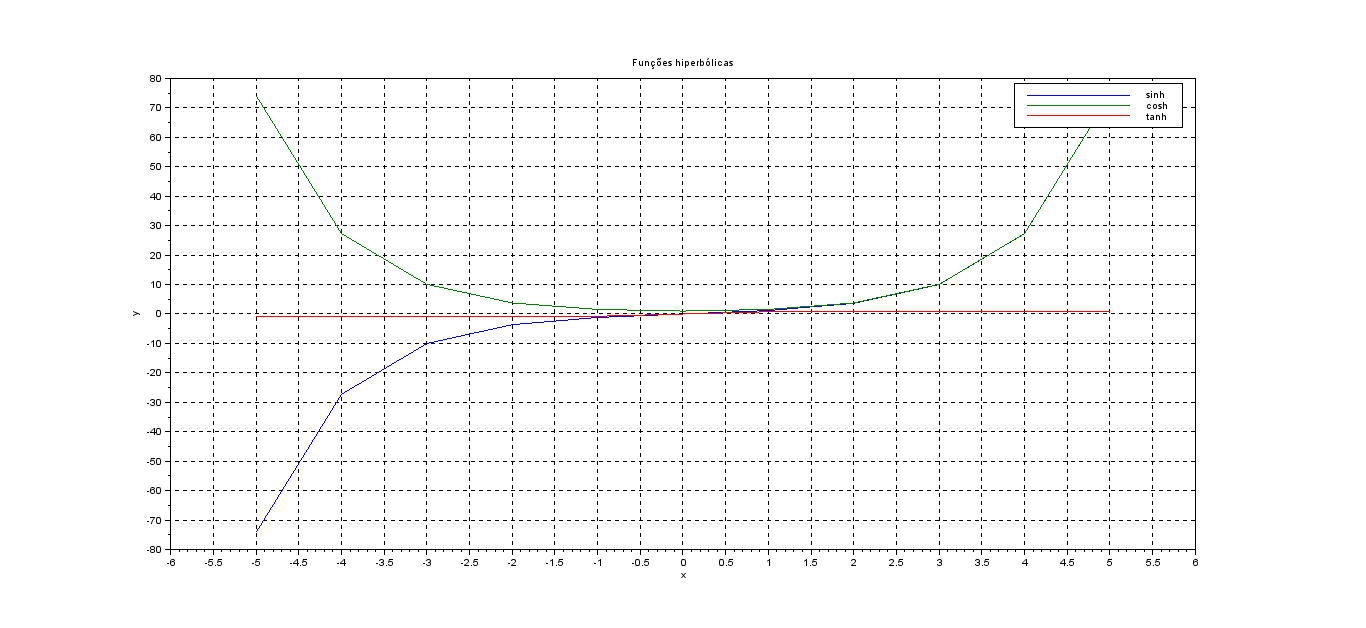
\includegraphics[width=0.99\linewidth]{images/hiperbolicas.png}

%   \tcblower
%   \solution
%   \lstinput{scilab}{listings/p09/hiperbolicas.sce}
% \end{task}

\end{document}

